This section presents the results of the significance study of the closeness centrality based on the described hypotheses.

Table \ref{tab:1} shows a summary of our data that we are going to use to test our hypothesis. We can observe that the different SDN have a wide range of number of nodes. There is small networks such as Basque with around 12k nodes and big networks like Czech with almost 70k nodes. All the networks are sparse, the density of edges is low. Despite its sparsity, the mean degrees are quite different with some cases around 4 and other around 13.

\begin{table}[!htb]
    \centering
    \begin{tabular}{l c c c c} \toprule
        \textbf{Language} & \textbf{\#Nodes} ($N$) & \textbf{\#Edges} ($E$) & \textbf{Mean degree} ($k$) & \textbf{Density of edges} ($\delta$) [$10^{-4}$]  \\ \midrule
         Arabic & 21532 & 68743 & 6,39 & 2,97 \\ 
         Basque & 12207 & 25541 & 4,19 & 3,42 \\
         Catalan & 36865 & 195075 & 10,69 & 2,90 \\ 
         Chinese & 40298 & 180925 & 8,98 & 2,23\\ 
         Czech & 69303 & 257254 & 7,42 & 1,01 \\ 
         English & 29634 & 193078 & 13,03 & 4,40 \\ 
         Greek & 13283 & 43961 & 6,62 & 4,98 \\ 
         Hungarian & 36126 & 106681 & 5,91 & 1,63 \\ 
         Italian & 14726 & 55954 & 7,60 & 5,16 \\
         Turkish & 20409 & 45625 & 4,47 & 2,19 \\ \bottomrule
    \end{tabular}
    \caption{Summary of the properties of the degree sequences of the studied languages.}
    \label{tab:1}
\end{table}

In order to study the importance of the network closeness centrality, we want to evaluate if this metric is significantly large with regard our random graph models (our null hypothesis). Therefore, we obtained experimentally which is the probability of the closeness centrality of the random graph to be greater than the input graph, $P(\mathcal{C}_{NH} \geq \mathcal{C}) \approx \frac{1}{T}f(\mathcal{C}_{NH} \geq \mathcal{C}) \leq \alpha$. Table \ref{tab:2} shows that our null hypothesis is correct. Our networks have a closeness centrality larger than our null hypothesis models.

\begin{table}[!htb]
    \centering
    \begin{tabular}{l c c c} \toprule
        \textbf{Language} & \textbf{Closeness Centrality} & \textbf{p-value (Binomial)} & \textbf{p-value (Switching)} \\ \midrule
Arabic & 0.32597 & 0 & 0 \\ 
Basque & 0.26981 & 0 & 0 \\ 
Catalan & 0.34222 & 0 & 0 \\ 
Chinese & 0.32564 & 0 & 0 \\ 
Czech & 0.30661 & 0 & 0 \\ 
English & 0.34381 & 0 & 0 \\ 
Greek & 0.31403 & 0 & 0 \\ 
Hungarian & 0.28971 & 0 & 0 \\ 
Italian & 0.32763 & 0 & 0 \\ 
Turkish & 0.36075 & 0 & 0 \\  \bottomrule 
    \end{tabular}
    \caption{Summary of the obtained p-values for the experiemnts performed.}
    \label{tab:2}
\end{table}

Figure \ref{fig:closeness_distribution} shows the obtained results for closeness centrality computation for both models. It is clear that the performance of both studied models is very different; all results for the Binomial model lie further from the measure than those obtained with the Switching model. Other interesting characteristics are revealed by the plot; the variance of the obtained results is not the same for all languages. Observe, for instance, how Basque presents a cloud of points more spread than Catalan, both for the Binomial and Switching models. This probably can be explained by the fact that the number of edges is smaller and therefore the metric is less stable.
\begin{figure}[!htp]
    \centering
    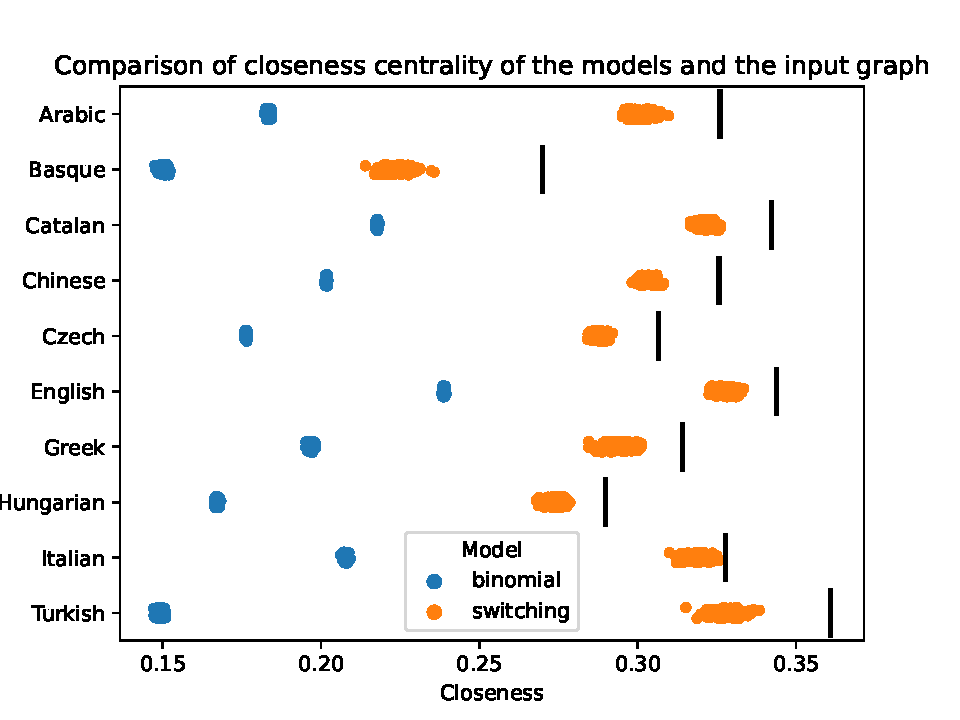
\includegraphics[width=0.5\textwidth]{figures/closeness_distribution.pdf}
    \caption{Distribution of the closeness centrality of the different models and the input graph }
    \label{fig:closeness_distribution}
\end{figure}